\documentclass[russian, 10pt]{beamer}

\beamertemplatenavigationsymbolsempty

\usepackage[utf8]{inputenc}
\usepackage[russian]{babel}

\usepackage{textcomp}
\usepackage{bm}
\usepackage{caption}
\usepackage{subfig}
\usepackage{listings}
\usepackage{hyperref}
\usepackage{pgfplots}
\usepackage{tikz}
\usepackage{amsthm}
\usepackage{pgf,pgfarrows,pgfnodes}
\usepackage{amsmath}
\usepackage{amsfonts}
\usepackage{amssymb}
\usepackage{wrapfig}
\usepackage{indentfirst}
\usepackage{setspace}
\usepackage{graphicx}
\usepackage{textcomp}
\usepackage{array}
\usepackage{verbatim}



\DeclareMathOperator{\E}{\mathbb{E}}
\DeclareMathOperator{\D}{\mathbb{D}}
\DeclareMathOperator{\R}{\mathbb{R}}


\usepackage{graphicx}
\usepackage[linesnumbered]{algorithm2e}


\begin{document}

\begin{frame}
\centering
\textsc{\textcolor{black}{Eugen Bobrov}}\\[2mm]

\includegraphics[scale=0.35]{images/2.png}
\end{frame}

\begin{frame}
В обучающей выборке есть один магазин, которого нет в тестовой. Его последовательность крайне мала -- всего 5 записей. Тогда как медиана длин последовательностей равна 180. Небходимо исключить его из обучающей выборки:

\begin{itemize}

\item idFilial = 15
\item idSubGrp = 1
\item KanalDB = 1

\end{itemize}

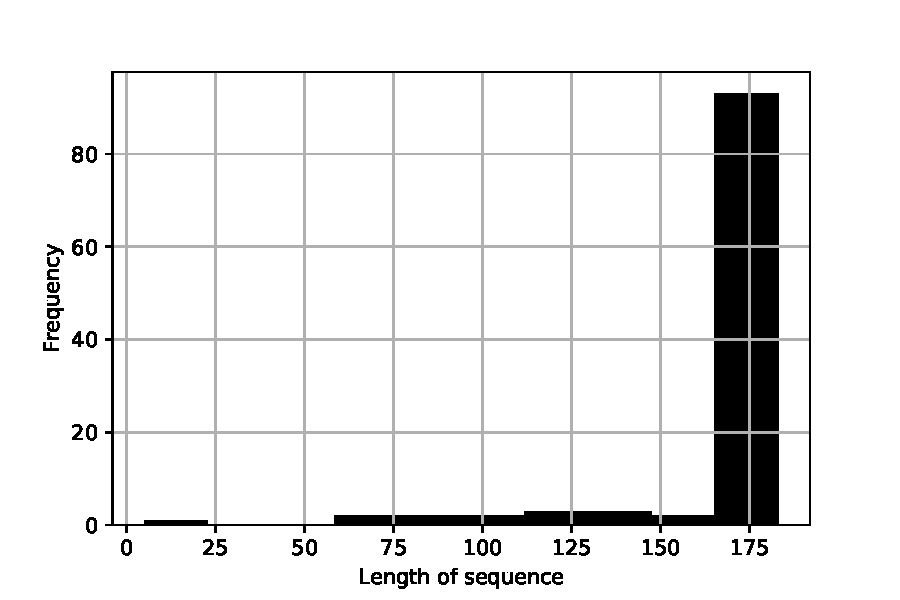
\includegraphics[scale=0.5]{images/sizes.pdf}
\end{frame}


\begin{frame}
Длины последовательностей обучающей выборки:
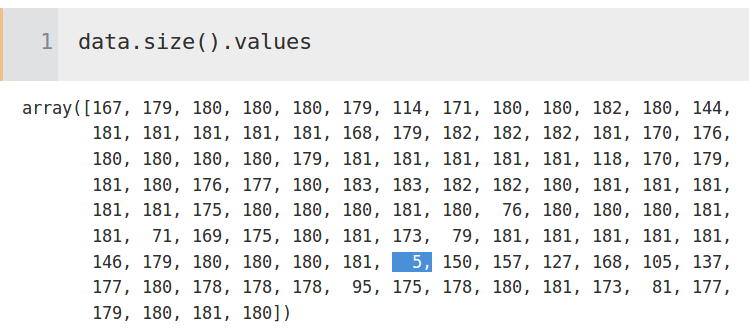
\includegraphics[scale=0.4]{images/6.png}
\end{frame}

\begin{frame}

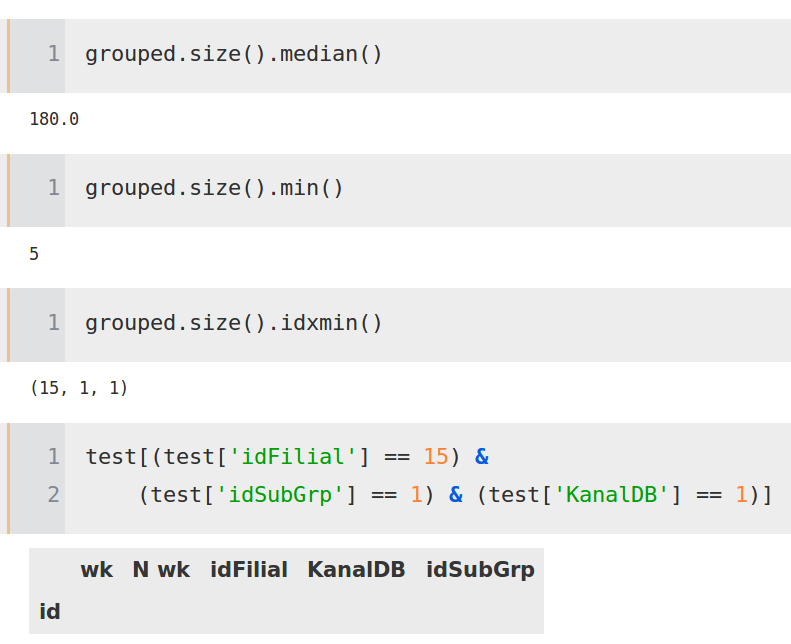
\includegraphics[scale=0.4]{images/7.png}
\end{frame}

\begin{frame}
Достаточно вставить следующий код:
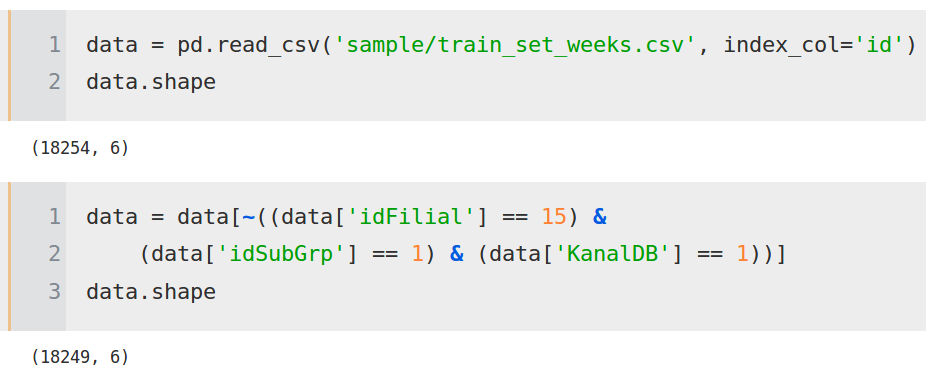
\includegraphics[scale=0.35]{images/8.png}
\end{frame}



\end{document}